% Jabuti 1.0 Manual
%
%     Copyright 2003  Auri Marcelo Rizzo Vicenzi, M�rcio Eduardo Delamaro,
%                     Jos� Carlos Maldonado
%
%      Permission is granted to copy, distribute and/or modify this
%      document under the terms of the GNU Free Documentation License,
%      Version 1.3 or any later version published by the Free Software
%      Foundation; with no Invariant Sections, no Front-Cover Texts and
%      no Back-Cover Texts.  A copy of the license is included in the
%      section entitled "GNU Free Documentation License".
%
%      A copy of license terms is also found in the file FDL.TXT


\documentclass[a4paper,11pt]{article}

%----------------------Packages------------------------------------------------
\usepackage{ae}
\usepackage{subfigure}
\usepackage{setspace}
\usepackage{float}
\usepackage{color}
\usepackage{verbatim}
\usepackage{multirow}
\usepackage{graphicx}
%\usepackage[dvipdfm]{graphicx}
\usepackage{xspace}
\usepackage{url}
\usepackage[nottoc]{tocbibind}
\usepackage[T1]{fontenc}
\usepackage[verbose,left=20mm,right=20mm,top=20mm,bottom=20mm]{geometry}

\usepackage{titlesec}
\usepackage{colortbl}

\usepackage{afterpage}
\usepackage{fancyvrb}
\usepackage{icmcheader}

%------------------------------------------------------------------------------

%----------------------General Definitions-------------------------------------
\input{macros.tex}
%------------------------------------------------------------------------------

\begin{document}
%-------------------Cabe�alho-------------------------------------------
\secao{DEPARTAMENTO DE CI�NCIAS DE COMPUTA��O E ESTAT�STICA}
\subsecao{Caixa Postal 668 -- CEP 13560-970 -- S�o Carlos, SP --
Fone (16) 273-9655 -- Fax (16) 273-9751}

\makeicmcheader

\vspace*{3cm}

\begin{center}
%\renewcommand{\thefootnote}{\fnsymbol{footnote}}
{\noindent\normalfont \LARGE\bfseries \toolname\ -- Java Bytecode} \\
{\noindent\normalfont \LARGE\bfseries Understanding and Testing} \\

\vspace*{0.5cm}

\begin{figure}[!ht]
\begin{center}

\includegraphics[width=5cm]{fig/jabuti.eps}
\end{center}
\end{figure}

{\noindent\normalfont\large\bfseries User's Guide}\\
{\noindent\normalfont Version 1.0 -- Java}

\vspace*{0.5cm}

A. M. R. Vincenzi$^{\dag}$,
%W.  E.  Wong$^{\S}$,
M.  E.  Delamaro$^{\ddag}$ and
J.  C.  Maldonado$^{\dag}$
 \\[0.5cm]

{\small
{$^\dag$Instituto de Ci\^encias Matem\'aticas e de Computa\c c\~ao}\\
{Universidade de S\~ao Paulo}\\
{S\~ao Carlos, S\~ao Paulo, Brazil}\\
{\tt \{auri, adenilso, jcmaldon\}@icmc.usp.br}\\[0.5cm]
%-------------------------------------------------------------
%% \begin{minipage}{0.45\textwidth}
%% \centering
%% {$^\S$Department of Computer Science} \\
%% {University of Texas at Dallas} \\
%% {Richardson, Texas, USA} \\
%% {\tt ewong@utdallas.edu}\\
%% \end{minipage}
%-------------------------------------------------------------
%%\hfill
\begin{minipage}{0.45\textwidth}
\centering
{$^\ddag$Faculdade de Inform\'atica}\\
{Centro Universit\'ario Eur\'ipides de Mar\'ilia}\\
{Mar\'ilia, S\~ao Paulo, Brazil}\\
{\tt delamaro@fundanet.br}\\
\end{minipage}
}
\vspace*{3cm}

\noindent{\normalfont \rmfamily S�o Carlos, SP, Brazil \\ March, 2003}\\[12pt]

\vfill{\footnotesize Copyright 2003  Auri Marcelo Rizzo Vicenzi, M�rcio Eduardo Delamaro, Jos� Carlos Maldonado}

\end{center}
\thispagestyle{empty}
\setcounter{page}{0}
%------------------------------------------------------------------------------

\frontmatter
\tableofcontents

%----------------------Abstract------------------------------------------------
\input{abstract}
%------------------------------------------------------------------------------
\onehalfspace
\mainmatter
%----------------------Introduction--------------------------------------------
%\input{introduction}
%------------------------------------------------------------------------------

%----------------------Background----------------------------------------------
%\input{background}
%------------------------------------------------------------------------------

%----------------------Example-------------------------------------------------
%\input{example}
%------------------------------------------------------------------------------

%----------------------Tool----------------------------------------------------
\input{tool}
%------------------------------------------------------------------------------

%----------------------Session Creation----------------------------------------
\input{project}
%------------------------------------------------------------------------------

%----------------------Coverage Analysis---------------------------------------
\input{coverage}
%------------------------------------------------------------------------------

%----------------------Slice---------------------------------------------------
\input{slicing}
%------------------------------------------------------------------------------

%----------------------Slice---------------------------------------------------
\input{metrics}
%------------------------------------------------------------------------------

\afterpage{\clearpage}
\newpage

%----------------------  Mobile devices ----------------------------------------
%% This is part of the Jabuti 1.0 Manual.
% Copyright 2003 (c) Auri Marcelo Rizzo Vicenzi, Marcio Eduardo Delamaro,
% Jose Carlos Maldonado.
% See the file FDL.TXT for copying conditions.

\section{\toolname em dispositivos m�veis}
A ferramenta \toolname foi adaptada para ser utilizada
no teste de programas Java que rodam em dispositivos
m�veis como PDAs ou telefones celulares. Mais precisamente,
que est�o de acordo com o perfil MIDP (Mobile Information
Device Profile).

Essa se��o descreve as diferen�as na utiliza��o da ferramenta para
o teste desse tipo de software. As mudan�as de procedimento dizem
respeito, principalmente, � instrumenta��o e execu��o dos casos de
teste. Como os programas instrumentados devem executar em
dispositivos m�veis,\footnote{Quando nos referimos a dispositivos m�veis
inclu�mos os simuladores que, apesar de executarem no desktop, est�o
sujeitos aos mesmos tipos de limita��es do perfil MIDP.} o tipo de
instrumenta��o deve ser adequada �quele ambiente. Al�m disso, os
dados de execu��o (trace) devem ser analisados pela \toolname, no
desktop.

Assim, a primeira mudan�a a ser feita � a instala��o de um
servidor que vai ser respons�vel pela aquisi��o dos dados de
execu��o dos programas e a gera��o do arquivo de trace que �
tratado pela \toolname. O servidor pode ser instalado atrav�s de
um programa chamado diretamente na linha de comando ou de dentro
da pr�pria ferramenta.

Na chamada direta, o programa deve receber dois argumentos, como
mostra a descri��o abaixo:
\begin{verbatim}
> java -cp <classpath Jabuti> br.jabuti.device.ProberServer <port> <filename>
\end{verbatim}

O primeiro argumento indica o n�mero da porta � qual o servidor
vai se anexar. O segundo � o nome de um arquivo de configura��o
que descreve quais s�o os programas que devem ser tratados pelo
servidor. Um servidor pode tratar de mais de um programa em
execu��o ao mesmo tempo. O formato do arquivo de configura��o �
bastante simples. Ele possui, para cada programa a ser tratado,
duas linhas, contendo a identifica��o do programa e o nome do
arquivo de trace onde os dados de execu��o devem ser gravados.
Por exemplo:

\begin{verbatim}
PropExample
/home/user/Demos/PropExample.trc
Foo
/home/foo/foo.trc
\end{verbatim}

No arquivo de configura��o acima, dois programas poder�o ser
tratados pelo servidor. Um batizado de ```PropExample'' e outro
batizado de ``Foo''. Quando o servidor recebe dados de execu��o do
primeiro, esses dados ser�o gravados no arquivo
``/home/user/Demos/PropExample.trc'' e do segundo, no arquivo
``/home/foo/foo.trc''. Note que o nome do programa n�o est�
relacionado com a sess�o de teste criada para o teste. Esse nome �
atribu�do pelo testador no momento da instrumenta��o, como ser�
descrito adiante.

Um exemplo de utiliza��o do comando que instala o servidor seria:

\begin{verbatim}
java -cp Jabuti-bin.zip br.jabuti.device.ProberServer 1988 config.txt
\end{verbatim}

A instala��o atrav�s da ferramenta \toolname � feita atrav�s da
op��o ``Properties/Test Server''. Com essa opera��o abre-se a
janela mostrada na Figura~\ref{fig:testserver}. Nela o testador
deve selecionar a porta em que o servidor ser� instalado e o
arquivo de configura��o. Pode, tamb�m, editar esse arquivo e
salv�-lo, se necess�rio. O testador deve, ainda, selecionar a op��o
``Mobile device'', que indica o tipo de servidor desejado.

\begin{figure}[!ht]
\begin{center}
\includegraphics[width=0.50\textwidth]{fig/testserver.eps}
\caption{\label{fig:testserver}Instala��o do servidor para dispositivos
m�veis.}
\end{center}
\end{figure}

Outra diferen�a na execu��o da sess�o de teste para dispositivos
m�veis est� na instrumenta��o e do programa em teste e na execu��o
dos casos de teste. O programa � instrumentado e gera-se um
arquivo .jar contendo todas as classes que comp�em o programa,
instrumentando-se aquelas que foram escolhidas na cria��o do
projeto de teste. O comando que realiza a instrumenta��o � o
seguinte:

\begin{verbatim}
java -cp <classpath Jabuti> br.jabuti.device.ProberInstrum <op��es> <classe base>
\end{verbatim}

A classe base refere-se ao nome da classe do MIDlet que se deseja
testar. Deve-se notar que num �nico ``pacote'' � poss�vel
colocar-se diversos MIDlets distintos. Por�m, somente um pode ser
instrumentado de cada vez. As op��es de instrumenta��o s�o as
seguintes:

\begin{description}
\item [<-d diret�rio>:] indica o diret�rio no qual se encontra o
arquivo de projeto. � opcional e, se n�o for fornecido, assume-se
o diret�rio corrente;
\item[<-p projeto>:] nome do arquivo de projeto, criado pela
\toolname, que corresponde � sess�o de teste. Argumento
obrigat�rio;
\item[<-o arquivo>:] d� o nome do arquivo .jar onde ser�o
gravadas as classes instrumentadas do programa. Como as classes
instrumentadas fazem chamadas a m�todos localizados em classes da
\toolname, essas classes s�o, tamb�m, adicionadas ao arquivo de
sa�da;
\item [<-name midlet id>:] � o nome que ser� dado ao programa em
teste. � esse nome que identifica o MIDlet para o servidor de
teste, como visto anteriormente;
\item [<-h end. servidor>:] esse par�metro fornece o endere�o
onde o servidor de teste foi instalado, no formato
``128.123.82.71:1988'' ou ``myserver.com.br:1988''. � um par�metro
opcional. Caso n�o seja fornecido, os dados n�o ser�o enviados a
nenhum servidor. N�o utilizar essa op��o torna a execu��o do
programa in�til em termos de teste, propriamente dito, mas pode
ser �til para a depura��o da ferramenta. Os dados de teste podem
ser exibidos na sa�da padr�o ou num arquivo, como ser� visto a
seguir;
\item [<-temp arquivo>:] utiliza o arquivo especificado como
dep�sito tempor�rio dos dados de trace, no dispositivo. Isso
permite que, em dispositivos que possuem sistema de arquivos, os
dados fiquem armazenados ali, salvando espa�o na mem�ria
principal. O nome ``\_\_STDOUT\_\_'' indica que os dados devem ser
escritos na sa�da padr�o do didpositivo m�vel. Isso s� faz sentido se a
execu��o for feita num simulador no desktop, poi, em geral os
dispositivos m�veis n�o apresentam resultados na sa�da padr�o;
\item [<-mem valor>:] especifica um threshold de mem�ria
dispon�vel que deve ser respeitado para armazenamento dos dados de
trace. Quando a quantidade de mem�ria cai abaixo desse valor os
dados s�o enviados para o servidor de teste, ou armazenados no
arquivo tempor�rio. O valor pode ser dado em bytes (por exemplo,
1024), em kbytes ou em mbytes (por exemplo, 128K ou 3M). � um
par�metro opcional e, se n�o fornecido, assume o valor zero,
indicando que n�o existe threshold e os dados s�o sempre
armazenados, at� que a execu��o termine;
\item [<-nokeepalive>:] se utilizado, esse par�metro indica que a
conex�o (TCP) entre o dispositivo e o servidor de teste n�o deve
ser mantida durante toda a execu��o do programa. Assim, cada vez
que dados devem ser transmitidos, uma nova conex�o � criada. Isso
pode representar economia nos dispositivos em que a utiliza��o de
rede � cara e paga em fun��o do tempo de utiliza��o. A utiliza��o
da op��o ``<-temp arquivo>'' j� determina que a conex�o n�o
ser� mantida viva pois todos os dados de execu��o s�o gravados no
arquivo tempor�rio e somente no final da execu��o do MIDlet os
dados s�o enviados ao servidor.
\end{description}

Seguem-se alguns exemplos da utiliza��o do instrumentador, com
alguma combina��es de par�metros. \\

\hrule
\begin{verbatim}
java -cp Jabuti-bin.zip br.jabuti.device.ProberInstrum -name PropExample
-p Propexample.jbt -o PropExample.jar -h 200.188.151.130:2000 example.PropExample
\end{verbatim}

Nesse exemplo, o programa, cuja sess�o de teste est� descrita no
projeto chamado ``PropExample'', recebeu o nome de
``PropExample'', que tamb�m � o nome dado ao arquivo .jar de
sa�da. Os dados de trace ser�o enviados ao endere�o
``200.188.151.130:2000'' e a classe do MIDlet �
``example.PropExample''. Como n�o foi estabelecido um threshold
de mem�ria, todos os dados ser�o armazenados e somente enviados no
final da execu��o do programa. Mesmo assim, a conex�o entre o
dispositivo e o servidor de teste � aberta no in�cio da execu��o
do MIDlet e permanece aberta at� o final do envio dos dados. \\

\hrule
\begin{verbatim}
java -cp Jabuti-bin.zip br.jabuti.device.ProberInstrum -name PropExample
-p Propexample.jbt -o PropExample.jar -h 200.188.151.130:2000 -nokeepalive
example.PropExample
\end{verbatim}

O mesmo do exemplo anterior, por�m a conex�o n�o permanece aberta
o tempo todo. Ela s� � criada no in�cio da execu��o, para que seja verificada
se realmente pode ser criada e depois, no final, quando os dados
forem enviados. \\

\hrule
\begin{verbatim}
java -cp Jabuti-bin.zip br.jabuti.device.ProberInstrum -name PropExample
-p Propexample.jbt -o PropExample.jar -h 200.188.151.130:2000 -nokeepalive
-mem 512M example.PropExample
\end{verbatim}

Nesse caso, os dados s�o enviados periodicamente, quando a
quantidade de mem�ria dispon�vel estiver abaixo do valor
estabelecido, ou seja 512 mega-bytes. Como � improv�vel que algum
dispositivo tenha uma mem�ria livre desse tamanho, o que deve
ocorrer � que a cada dado de trace coletado, este seja
imediatamente enviado para o servidor. Como a op��o
``-nokeepalive'' foi utilizada, isso significa que a cada dado
coletado, uma nova conex�o � criada, o que pode interferir
sobremaneira na execu��o do MIDlet. \\

\hrule
\begin{verbatim}
java -cp Jabuti-bin.zip br.jabuti.device.ProberInstrum -name PropExample
-p Propexample.jbt -o PropExample.jar -h 200.188.151.130:2000 -nokeepalive
-temp /root1/temp.txt example.PropExample
\end{verbatim}

Com a utiliza��o do arquivo tempor�rio, os dados de trace s�o
sempre enviados para esse arquivo e somente no final enviados para
o servidor. Assim n�o s�o criadas, constantemente, conex�es.\\

\hrule
\begin{verbatim}
java -cp Jabuti-bin.zip br.jabuti.device.ProberInstrum -name PropExample
-p Propexample.jbt -o PropExample.jar -temp __STDOUT__ example.PropExample
\end{verbatim}

Os dados de teste coletados s�o apresentados na sa�da padr�o do
dispositivo. Como n�o foi fornecido o threshold de mem�ria esse
resultado s� � apresentado no final da execu��o. \\

\hrule
\ \\

Depois de instrumentadas as classes, � necess�rio ainda mais um
passo para que o programa possa ser executado. � a pr�-verifica��o
do bytecode e o empacotamento num �nico arquivo. Isso � feito com
o comando descrito a seguir:

\begin{verbatim}
> java -cp <classpath Jabuti> br.jabuti.device.Preverify <op��es>
\end{verbatim}

Os argumentos fornecidos para a execu��o s�o os seguintes:

\begin{description}
\item [<-source arquivo>:] esse argumento � obrigat�rio e indica
qual � o arquivo .jar onde est�o as classes originais do programa
a ser carregado no dispositivo m�vel. Note-se que, como comentado
anteriormente, esse arquivo pode conter diversos MIDlets, al�m
daquele sendo testado;
\item [<-instr arquivo">:] � o nome do arquivo .jar que foi criado
no passo anterior, a instrumenta��o. O que o programa ir� fazer �
substituir no arquivo original, as classes que foram
instrumentadas, mantendo as demais como est�o;
\item[<-o arquivo>:] indica o nome do arquivo .jar de sa�da. � um
argumento opcional e, caso n�o seja fornecido, assume-se o mesmo
nome do arquivo original. Nesse caso, o arquivo original �
sobrescrito;
\item [<-jad arquivo>:] especifica o nome do arquivo .jad
a ser gerado, com as informa��es sobre o ``pacote'' gerado. �
opcional e, se n�o for fornecido, nada � gerado;
\item [<-WTK diret�rio>:] a \toolname n�o realiza a pr�-verifica��o
por si s�. Ela utiliza o toolkit de desenvolvimeto wireless da SUN
para efetuar tal tarefa. Por isso, o testador deve indicar qual �
o diret�rio onde encontra-se o WTK.
\end{description}

Um exemplo de sua utiliza��o seria:

\begin{verbatim}
java -cp Jabuti-bin.zip br.jabuti.device.Preverify -source Demos.jar
-instr PropExample.jar -o Demos.jar -jad Demos.jad -WTK /home/user/WTK22
\end{verbatim}

Conclu�do esse passo, o programa est� pronto para ser executado
num simulador ou dispositivo m�vel. Os dados, dependendo do tipo
de instrumenta��o, pode ser enviado ao servidor selecionado ou
simplesmente escrito num arquivo tempor�rio. Deve-se notar que na
maioria dos dispositivos, o usu�rio deve fornecer autoriza��o para
algumas opera��es privilegiadas como a cria��o de uma conex�o de
rede ou leitura/escrita de arquivos. Por isso, a instrumenta��o
pode alterar o comportamento do
MIDlet, fazendo com que o programa seja interrompido e tal
autoriza��o solicitada. Isso por�m, n�o deve representar problema
pois, ap�s a exibi��o de uma janela de solicita��o de autoriza��o,
como a da Figura~\ref{fig:autoriza}, o programa segue normalmente.

Para se executar o programa utilizando o simulador do WTK pode-se
utilizar o comando:

\begin{verbatim}
/home/user/WTK22/bin/emulator.exe -Xdescriptor:Demos.jad
\end{verbatim}

\begin{figure}[!ht]
\begin{center}
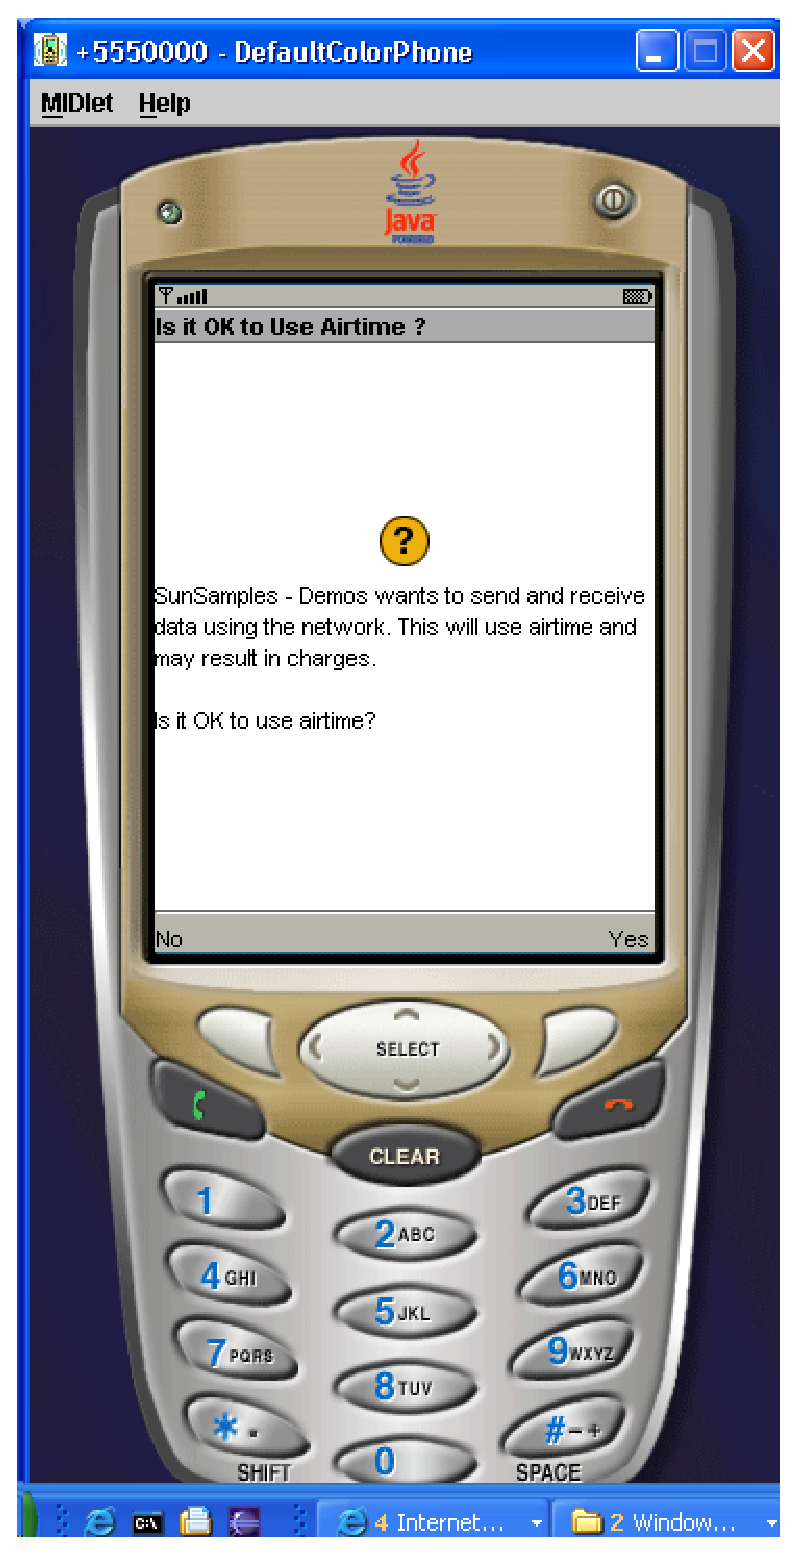
\includegraphics[width=0.30\textwidth]{fig/autoriza.eps}
\caption{\label{fig:autoriza}Execu��o no emulador: autoriza��o para criar conex�o.}
\end{center}
\end{figure}

%------------------------------------------------------------------------------


%----------------------JaBUTi Evolution----------------------------------------
%\input{evolution}
%------------------------------------------------------------------------------

%----------------------Acknowledgments-----------------------------------------
%% This is part of the Jabuti 1.0 Manual.
% Copyright 2003 (c) Auri Marcelo Rizzo Vicenzi, Marcio Eduardo Delamaro,
% Jose Carlos Maldonado.
% See the file FDL.TXT for copying conditions.

\section*{Acknowledgments}
The authors would like to thank the Brazilian Funding Agencies --
CNPq, FAPESP and CAPES -- and the Telcordia Technologies (USA) for
their partial support to this research. The authors would also
like to thank the creators of the turtle image used as symbol of
\toolname found at \url{http://www.indiancanyonvillage.org/}.

%------------------------------------------------------------------------------

\newpage

\section{License}

%\begin{verbatim}
%\input{FDL.TXT}
%\end{verbatim}

{\footnotesize
\verbatiminput{FDL.TXT}
}

\newpage

\singlespace
%----------------------Bibliografia--------------------------------------------
%\bibliographystyle{plain}
%\bibliography{../../../bib/auri,../../../bib/others}
\input{biblio}
%------------------------------------------------------------------------------
\end{document}
